\documentclass{article}
\usepackage[paperwidth=7.10in,paperheight=2.35in,margin=0in]{geometry}
\usepackage{tikz}
\usepackage{amsmath,amssymb}
\usetikzlibrary{arrows.meta,calc,decorations.pathmorphing,positioning}
\pagestyle{empty}
\definecolor{ink}{HTML}{17233A}
\definecolor{blue}{HTML}{2563A6}
\definecolor{red}{HTML}{B23A48}
\definecolor{green}{HTML}{27836B}
\definecolor{gold}{HTML}{B7791F}
\definecolor{pale}{HTML}{F3F6FA}
\begin{document}
\noindent
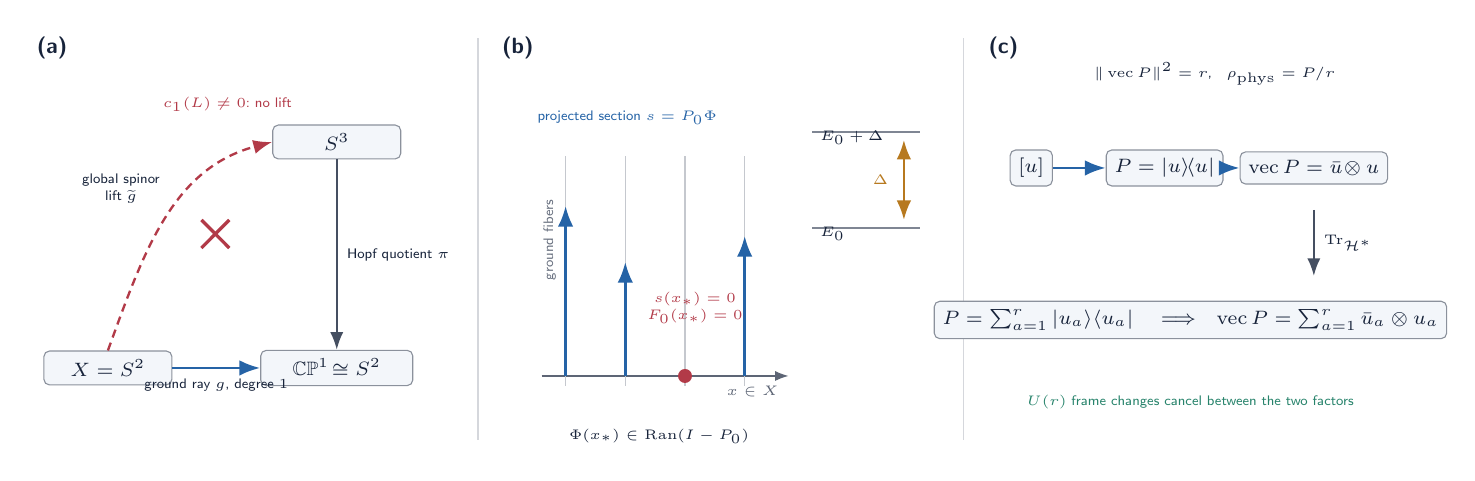
\begin{tikzpicture}[x=.995in,y=1in,>=Latex,font=\sffamily\scriptsize,text=ink,
  box/.style={draw=ink!50,rounded corners=2pt,fill=pale,inner sep=3pt,align=center},
  flow/.style={->,line width=.75pt,draw=ink!80},
  blueflow/.style={->,line width=1pt,draw=blue}]

% panel dividers
\draw[ink!18] (2.34,.16)--(2.34,2.17);
\draw[ink!18] (4.78,.16)--(4.78,2.17);

% (a) Hopf lifting diagram
\node[font=\sffamily\bfseries\footnotesize] at (.20,2.12) {(a)};
\node[box,minimum width=.64in] (x) at (.48,.52) {$X=S^2$};
\node[box,minimum width=.76in] (cp) at (1.63,.52) {$\mathbb{CP}^{1}\!\cong S^2$};
\node[box,minimum width=.64in] (s3) at (1.63,1.65) {$S^3$};
\draw[blueflow] (x)--node[below,font=\sffamily\tiny] {ground ray $g$, degree $1$} (cp);
\draw[flow] (s3)--node[right,font=\sffamily\tiny] {Hopf quotient $\pi$} (cp);
\draw[->,densely dashed,line width=.85pt,draw=red] (x.north) to[out=70,in=195]
  node[pos=.53,above left,font=\sffamily\tiny,align=center] {global spinor\\lift $\widetilde g$} (s3.west);
\draw[red,line width=1.2pt] (1.02,1.19)+(-.07,-.07)--+(.07,.07);
\draw[red,line width=1.2pt] (1.02,1.19)+(-.07,.07)--+(.07,-.07);
\node[red,font=\sffamily\tiny,align=center] at (1.08,1.84) {$c_1(L)\ne0$:\ no lift};

% (b) forced zero and gap (fiber schematic, not a sampled curve)
\node[font=\sffamily\bfseries\footnotesize] at (2.54,2.12) {(b)};
\draw[->,ink!70] (2.66,.48)--(3.90,.48) node[below left,font=\sffamily\tiny] {$x\in X$};
\foreach \xx in {2.78,3.08,3.38,3.68}{\draw[ink!25] (\xx,.43)--(\xx,1.58);}
\draw[blueflow] (2.78,.48)--(2.78,1.33);
\draw[blueflow] (3.08,.48)--(3.08,1.05);
\fill[red] (3.38,.48) circle (.035);
\draw[blueflow] (3.68,.48)--(3.68,1.18);
\node[blue,align=center,font=\sffamily\tiny] at (3.09,1.77) {projected section $s=P_0\Phi$};
\node[red,align=center,font=\sffamily\tiny] at (3.43,.82) {$s(x_*)=0$\\$F_0(x_*)=0$};
\node[ink!65,font=\sffamily\tiny,rotate=90] at (2.70,1.16) {ground fibers};
\draw[ink!55] (4.02,1.22)--(4.56,1.22);
\draw[ink!55] (4.02,1.70)--(4.56,1.70);
\node[right,font=\sffamily\tiny] at (4.01,1.19) {$E_0$};
\node[right,font=\sffamily\tiny] at (4.01,1.67) {$E_0+\Delta$};
\draw[<->,gold,line width=.9pt] (4.48,1.26)--(4.48,1.66);
\node[gold,left,font=\sffamily\tiny] at (4.45,1.46) {$\Delta$};
\node[align=center,font=\sffamily\tiny] at (3.25,.18) {$\Phi(x_*)\in\operatorname{Ran}(I-P_0)$};

% (c) gauge-cancelling projector lift
\node[font=\sffamily\bfseries\footnotesize] at (4.98,2.12) {(c)};
\node[box] (ray) at (5.12,1.52) {$[u]$};
\node[box] (proj) at (5.79,1.52) {$P=|u\rangle\!\langle u|$};
\node[box] (vec) at (6.54,1.52) {$\operatorname{vec}P=\bar u\!\otimes u$};
\draw[blueflow] (ray)--(proj);
\draw[blueflow] (proj)--(vec);
\node[box,minimum width=1.84in] (rankr) at (5.92,.76)
  {$P=\sum_{a=1}^{r}|u_a\rangle\langle u_a|$
   \quad$\Longrightarrow$\quad
   $\operatorname{vec}P=\sum_{a=1}^{r}\bar u_a\otimes u_a$};
\node[green,font=\sffamily\tiny,align=center] at (5.92,.35)
  {$U(r)$ frame changes cancel between the two factors};
\draw[flow] (6.54,1.31)--node[right,font=\sffamily\tiny] {$\operatorname{Tr}_{\mathcal H^*}$} (6.54,.98);
\node[font=\sffamily\tiny,align=center] at (6.04,1.99)
  {$\|\operatorname{vec}P\|^2=r$,\quad$\rho_{\rm phys}=P/r$};

\end{tikzpicture}
\end{document}
